\chapter[Lecture 15]{}\label{lec15}

\section*{Crystal Binding and elastic constants}

Structure $\to$ a game of Hard balls and/or mathematical puzzles.

$\Rightarrow$ Although the structure of crystals are described packing of hard balls. The real seenario is different. Otherwise one would as $k$ questions
\begin{itemize}
\itemsep=0pt
\item[(i)] Why all structures are not close packed?

\item[(ii)] Why $AB \ AB\ AB$ is stable giving $HCP$ and $ABC \ ABC\ldots$ FCC structures.

There could have been a random mixture!

\item[(iii)] What is that holds all the atoms together?

\item[(iv)] How does a crystal knows about axis system? 
\end{itemize}

There must be some attractive (may be electrostatic in nature) interactions that keeps the atoms together.

Gravitational force, Magnetic force affect the atoms significantly weekly to have effect of binding.

--- Bonds: exchange coupling, van der waals force, covalent bonding etc are under consideration.

\noindent
{\bf Cohesive energy:} Minimum energy need to be applied to the crystal to separate its' components into neutral free atoms at rest, at infinite separation.

\noindent
{\bf Lattice energy:} This term is used for ionic crystals - The minimum energy required to separate the components of a crystal to free atoms.
\begin{itemize}
\itemsep=0pt
\item[(a)] Inert gases are weakly bound: cohesive energy is a few percent of $c$, $S_{i}$, $Ge\ldots$ etc.

\item[(b)] Alkali metals have intermediate values of cohesive energy.

\item[(c)] Transition metals are strongly bound.
\end{itemize}

Melting point, Buck modulii depend/related to cohesive energy.

\section*{Inert gas crystals}
\begin{itemize}
\itemsep=0pt
\item Simplest crystal with electron distribution close to that of free atoms.

\item Transparent insulators, weakly bound, low melting point.

\item Atoms have very high ionization energy $\to$ electronic configuration is stable.

\item Outermost cells are completely filled, electron distribution is spherically symmetric.

\item Form in close packed structure (FCC) except $He^{3}$ and $He^{4}$
\begin{itemize}
\itemsep=0pt
\item[(i)] $He^{3}$ and $He^{4}$ do not solidify at zero pressure even at absolute zero. Zero-point motion is a quantum effect that plays dominant role for $He^{3}$ and $He^{4}$.

\item[(ii)] Average fluctuation at $OK$ is 30\% to 40\% of bond length. Excluding zero-point energy, molar volume = 90 cc/mole for solid $He$. Experimental value 27.5 cc/mole for liquid $He^{4}$ and 36.8 cc/mole for liquid $He^{3}$.
\end{itemize}
What holds the atoms together:
\end{itemize}

\section*{Van der Waals-London Interaction}

If the charge distribution is rigit, interaction would be zero $\to$ spherical distribution of electrons makes total charge zero outside neutral atom (electrons + nucleus). So cohesive energy $\hookrightarrow 0$. But in reality, atoms can induce dipole moment between them.
\begin{figure}[H]
\centering
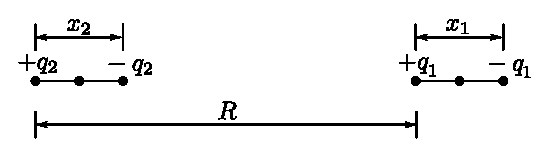
\includegraphics{images/lecture15/fig1.eps}
\end{figure}

For similar atoms one can assume $q_{1}=a_{2}=q$.

$\therefore$ The Hamiltonian of the unperturbed system will be
\begin{equation*}
H_{0}=\dfrac{P^{2}_{1}}{2m}+\frac{1}{2}Cx^{2}_{1}+\dfrac{P^{2}_{2}}{2m}+\frac{1}{2}Cx^{2}_{2}\tag{1}\label{lec15-eq1}
\end{equation*}
\begin{quote}
$C=mw^{2}_{0} =$ force constant.

$W_{0} =$ strongest optical absorption if uncoupled atoms.
\end{quote}
Switch on interaction between them
\begin{equation*}
H_{1}=\dfrac{q^{2}}{R}+\frac{q^{2}}{R+x-x_{2}}-\frac{q^{2}}{R+x_{1}}-\frac{q^{2}}{R-x_{2}}\tag{2}\label{lec15-eq2}
\end{equation*}
For
\begin{equation*}
|x_{1}|,|x_{2}|<< R \fbox{$H_{1}=\dfrac{2q^{2}x_{1}x_{2}}{R^{3}}$}\tag{3}\label{lec15-eq3}
\end{equation*}
Consider normal mode transformation as
\begin{equation*}
x_{s}=\dfrac{1}{\sqrt{2}}(x_{1}+x_{2})\quad x_{a}=\dfrac{1}{\sqrt{2}}(x_{1}-x_{2})\tag{4}\label{lec15-eq4}
\end{equation*}
\begin{align*}
\therefore\quad &\fbox{$x_{1}=\dfrac{x_{s}+x_{a}}{\sqrt{2}}$}\quad \fbox{$x_{2}=\dfrac{x_{s}-x_{a}}{\sqrt{2}}$}\\
\therefore\quad &p_{1}=\dfrac{p_{s}+p_{a}}{\sqrt{2}}\quad p_{2}=\dfrac{p_{S}-p_{a}}{\sqrt{2}}
\end{align*}
$\therefore$ The total Hamiltonian will be $H=H_{0}+H_{1}$
$$
\therefore\quad H=\left[\dfrac{p^{2}_{s}}{2m}+\frac{1}{2}\left(C-\frac{2q^{2}}{R^{3}}\right)x^{2}_{s}\right]+\left[\frac{pa^{2}}{2m}+\dfrac{1}{2}\left(C+\frac{2q^{2}}{R^{3}}\right)x^{2}_{a}\right]
$$
$\therefore$ Frequencies of the complied oscillators are
\begin{align*}
w &= \left[\left(c\pm \dfrac{2q^{2}}{R^{3}}\right)/m\right]^{\frac{1}{1}}=w_{0}\left[1\pm \frac{1}{2}\left(\frac{2q^{2}}{CR^{3}}\right)-\frac{1}{8}\left(\frac{2q^{2}}{CR^{3}}\right)^{2}+\cdots\right]\\
w_{0} &= \sqrt{\frac{c}{m}}
\end{align*}
$\therefore$ The zero point energy $=\dfrac{1}{2}\hbar(w_{s}+w_{a})$ which is smaller than $2\cdot \frac{1}{2}\hbar w_{0}$ by
$$
\Delta U=\frac{1}{2}\hbar (\Delta w_{s}+\Delta w_{a})=-\dfrac{\hbar w_{0}}{8}\left(\frac{2q^{2}}{CR^{3}}\right)^{2}\simeq -\frac{A}{R^{6}}
$$
This is called the {\em vander waal's interaction} also known as {\em London interaction} or {\em induced dipole - dipole interaction}.
\begin{itemize}
\item[(i)] This is purely a quantum effect $\Delta U=0$ for $\hbar=0$.

\item[(ii)] Does not depend on overlap of charge distribution of the atoms.

\item[(iii)] Does not depend on details of charge distribution.
\end{itemize}
For identical atoms $A\sim \hbar w_{0}\alpha^{2}$\quad $\alpha=$ Polarizability.

\section*{Repulsive Interaction}

As the two atoms are brought together, charge distribution gradually overlap, thereby changing electrostatic energy of the system.

When the separation is sufficiently small, repulsion starts to appear due to {\em Pauli Exclusion Principle} : two electrons cannot have all quantum numbers same.
\begin{figure}[H]
\centering
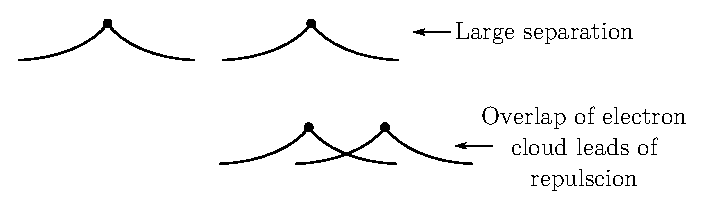
\includegraphics{images/lecture15/fig2.eps}
\end{figure}

Empirical formula for repulive potential $\sim \dfrac{B}{r^{12}}$

$\therefore$ Total energy
$$
\fbox{$U(r)=\dfrac{B}{r^{12}}-\dfrac{A}{r^{6}}$}
$$
$A$, $B$ are constants can be determined by measurements.

This is called Lennard - Jones potential.
$$
\text{Force } = -\dfrac{dU}{dr}
$$

Sometimes people use repulsive interaction as $\sim \lambda e^{\frac{-r}{\rho}}$
$$
\rho \to \text{ range of interaction.}
$$

\section*{Equillibrium Lattice Constants}

Lets consider $N$ atoms in the crystal.
$$
\therefore\quad U_{\text{tot}}\frac{1}{2}N(4t)\left[{\sum\limits_{j}}'\left(\dfrac{\sigma}{a_{ij}r}\right)^{12}-{\sum\limits_{j}}'\left(\dfrac{\sigma}{a_{ij}r}\right)^{6}\right]
$$
$\dfrac{1}{2}$' to avoid double counting.

\eject

$a_{ij}r$ is the distance between atom `$i$' and atom `$j$'

$r=$ nearest neighbour distance.

\smallskip

In FCC structure ${\sum\limits_{j}}'(a_{ij})^{-12}=12.13188$\quad ${\sum\limits_{j}}'(a_{ij})^{-6}=14.45392$

\smallskip

In FCC structure, no. of near neighbor $=12$ and the first term is close to 12.

\smallskip

In HCP structure ${\sum\limits_{j}}'(a_{ij})^{-12}=12.13229$\quad ${\sum\limits_{j}}'(a_{ij})^{-6}=14.45489$
\begin{align*}
\dfrac{dU_{tot}}{dr} &= -2N\epsilon \left[(12)\times (12.13)\cdot \dfrac{\sigma^{12}}{r^{13}}-(6)\cdot (14.4)\dfrac{\sigma^{6}}{r^{7}}\right]=0\\[3pt]
&\Rightarrow \left(\frac{r_{0}}{\sigma}\right)=1.09
\end{align*}
\begin{center}
\begin{tabular}{lcccc}
 & $N_{c}$ & $A_{r}$ & $K_{r}$ & $X_{e}$\\
Experimental value : $\dfrac{r_{0}}{\sigma}=$ & 1.14 & 1.11 & 1.1 & 1.09\\
\end{tabular}
\end{center}
Agreement is excellent.

$\therefore$ Cohesive energy at $T=OK$ and at Zero pressure
\begin{align*}
U_{tot} &= 2N\epsilon \left[12.13\left(\dfrac{\sigma}{r}\right)^{12}-14.45\left(\dfrac{\sigma}{r}\right)^{6}\right]\\[2pt]
&= (-2.15)(4N\epsilon)\quad \text{at } r=r_{0}
\end{align*}
Same for all inert gas. (calculated value)

\noindent
{\bf Quantum correction :} If the characteristic wavelength of the particle is $\lambda$, $p=\dfrac{h}{\lambda}$ $h\to$ planek's constant
$$
\text{K.E.} = \dfrac{P^{2}}{2M}=\dfrac{h^{2}}{2\lambda^{2}M}
$$
$\therefore$ Quantum zero point correction is inversely propertional to $M$. $\Rightarrow$ Reduce the binding by 28\%, 10\%, 6\% and 4\% for $N_{e}$, $A_{r}$, $K_{r}$ and $X_{e}$.

\bigskip

\noindent
{\bf N.B.}

Lattice constants of
$$
\left.
\begin{array}{l}
N_{e}^{20}=4.4644A^{0}\\[3pt]
N_{e}^{22}=4.4559A^{0}
\end{array}
\right\}
$$
at $2.5k$, higher mass particle has higher $k.E$. and hence more lattice expansion.

\eject

\section*{Ionic Crystals}

Made up of positive and negative ions. Bonding arises due to electrostatic interaction between oppositely charged atoms.

Ions have electronic configuration close to inert gases.

Charge distribution is close to spherical like inert gases.

\noindent
{\bf Quick estimate:} In NaCl, bond length $\sim 2.81A^{0}$.

$\to$ Coulomb part of potential energy $\sim 5.1 eV$

Experimental value of lattice energy $\sim 7.9 eV$/molecular unit comparable.

Since the long range interaction energy $\sim \dfrac{q}{f}$ is much stronger than the vander walls' energy $(\sim 1\%-2\%)$, the major contribution in attractive interaction is {\bf electrostatic coulomb potential}.

Repulsive energy may be considered similar like inert gas case. $\sim \lambda e^{-r_{ij}}/\rho$ 

$\lambda$ and $\rho$ are parameters.

Repulsion is short range in nature and will be considerable only from nearest neighbors. Ineration energy for $i^{\text{th}}$ atom will be
$$
\therefore\quad \fbox{$U_{i}=\sum\limits_{j\neq i}\lambda e^{\frac{-r_{ij}}{\rho}}\pm \sum\limits_{j\neq i}\dfrac{q^{2}}{r_{ij}}$}
$$
in SL unit $\dfrac{q^{2}}{r}\to \dfrac{q^{2}}{4\pi Gr}$

(+) sign for like charge and ($-$) sign for unlike charge.

\begin{example*}
NaCl\quad $U_{i}$ does not depend on whether atom `$i$' is

$Na$ or $Cl$\quad $U_{tot}=NU_{i}$ considering $N$ pairs.
\begin{align*}
U_{ij} &=
\left\{
\begin{array}{ll}
\lambda e^{\frac{-r_{0}}\rho}-\frac{q^{2}}{r_{0}} & \text{nearest neighbors}\\
\pm \frac{1}{n_{ij}}\frac{q^{2}}{r_{0}} & \text{other neighbors}
\end{array}
\right.\\
\therefore\quad U_{tot} &= N\left(Z\lambda e^{\frac{-r_{0}}{\rho}}-\dfrac{\alpha q^{2}}{r_{0}}\right)
\end{align*}
$Z=$ No. of nearest neighbors = Coordination No. (first)
$$
\alpha={\sum\limits_{j}}'\pm \frac{1}{n_{ij}}=\text{Madelung Constant}
$$
At equilibrium :
\begin{gather*}
N\dfrac{dU_{i}}{dr}=0=-\dfrac{Nz\lambda}{\rho}e^{\frac{-r_{0}}{\rho}}+\dfrac{N\alpha q^{2}}{r_{0}^{2}}\\
\text{or},\quad \fbox{$r^{2}_{0}e^{\frac{-r_{0}}{\rho}}=\rho\alpha \frac{q^{2}}{z\lambda}$}
\end{gather*}
$\therefore$ Equibrium separation is a function of $\rho$ and $\lambda$, and depend on many other parameters; $\alpha$, $q$ and $z$.

If $2N$ ions are there at their equillibrium distance,
$$
\fbox{$U_{tot}=-\frac{N\alpha q^{2}}{N_{0}}\left(1-\frac{\rho}{r_{0}}\right)$}
$$
The term \fbox{$-\dfrac{N\alpha q^{2}}{N_{0}}$} is called Madelung energy.
\end{example*}

Evaluation of {\bf Madelung Constant :} \fbox{$\alpha={\sum\limits_{j}}'\pm \dfrac{1}{n_{ij}}$}
$$
a, \frac{\alpha}{r_{0}}={\sum\limits_{j}}'\frac{1}{r_{j}}\quad r_{j}=n_{j}r_{0}
$$
For one dimensional chain
$$
\dfrac{\alpha}{r_{0}}=2\left(\frac{1}{r_{0}}-\frac{1}{2r_{0}}+\frac{1}{3r_{0}}-\cdots\right)
$$
`2' comes as there are two atoms on both sides.
\begin{gather*}
\text{or},\quad \alpha=2\left[1-\frac{1}{2}+\frac{1}{3}-\frac{1}{4}+\cdots\right]\\
l_{n}(1+x)=x-\frac{x^{2}}{2}+\frac{x^{3}}{3}-\frac{x^{4}}{4}\cdots\\
a, \fbox{$\alpha=2l_{n}2$}
\end{gather*}
In 3 dimension, it is difficult to write this (complex) one can arrange terms in such a way, the (+ve) and (-ve) terms nearly cancels each other.
\begin{center}
\begin{tabular}{lccc}
 & NaCl & C$_{s}$cl & Z$_{n}$S\\
$\alpha$ & 1.747565 & 1.762675 & 1.6381
\end{tabular}
\end{center}
\begin{figure}[H]
\centering
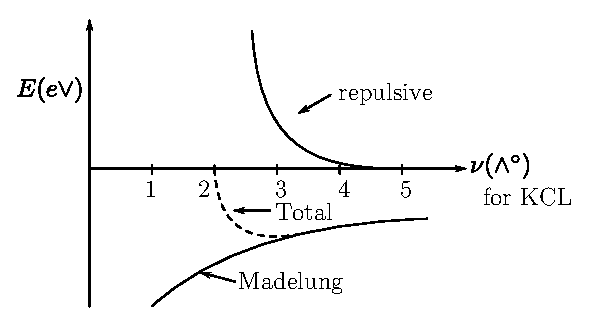
\includegraphics{images/lecture15/fig3.eps}
\end{figure}

\section*{Covalent Crystals}
\begin{itemize}
\item[$\to$] Bonding between two atoms involving a pair of electrons $\to$ homopolar bond in chemistry.

\item[$\to$] Bonds are very strong $\to$ bond strength comparable to the strength of ionic bonds.

\item[$\to$] Two electrons come from two participating atoms.

\item[$\to$] Prominent candidates.
\begin{quote}
Carbon $\to$ biology

Silicon $\to$ geology, semiconductor industry
\end{quote}

\item[$\to$] Bonds have directional property $\to$ structure has tetrahedral units (diamond structure) packing fraction $=0.34$. 
\end{itemize}
This is much smaller than the fraction of $0.74$ in fcc structure.
\begin{itemize}
\item[$\to$] Bonding depends on spin orientation, the spin-dependent coulomb energy is called {\em exchange interaction energy}.

\item[$\to$] Bond length of $cl_{2}$-is $\sim 2A^{0}$ while for $Ar$ it is $\sim 3.76A^{0}$.

\item[$\to$] Bonded electrons are shared by both the atoms.

\item[$\to$] Ionicity also plays some role in these systems if the bonding is between two different atoms.
\end{itemize}

\section*{Metals}
\begin{itemize}
\item[$\to$] High electrical conductivity.

\item[$\to$] Large number of conduction electrons. Interaction of conduction electrons with ion cores make large contribution in binding energy.

\item[$\to$] Lowering of energy of the valence electrons compared to free atom is the major contribution to binding.

\item[$\to$] Metals tend To crystallize in close packed structures.

hcp, fcc, bcc etc.
\end{itemize}

\section*{Hydrogen Bonds}
\begin{itemize}
\item[$\to$] A hydrogen may get attracted rather strongly by two atoms under certain condition.

\item[$\to$] Energy $\sim 0.1eV$ weak and largly ionic in character.

\item[$\to$] Forms with $F$, $O$, $N$ highly electro negative atoms.

example H$_{2}$O, ferro electric crystals, DNA etc.
\end{itemize}

Atomic radius $\to$ Highly debatable, depends on coordination no.

Sum of ionic radius of two dissimilar atom may not be equal to bond length usually a bit larger.
